
%%%%%%%%%%%%%%%%%%%%%%%%%%%%%%%%%%%%%%%%
%          Introduction
%%%%%%%%%%%%%%%%%%%%%%%%%%%%%%%%%%%%%%%%
The last century has seen great advancement of human transportation technology. whether it be wheeled vehicles running on the road, or submarines cruising the depth of seas, or rockets exploring the outer space. Human have not only conquered the land, but also the ocean, and even the space by enhancing our mobility using advanced vehicles. While these vehicles are fast, efficient and far-reaching, they all need highly structured media to work well. The Earth's most unstructured terrain still haven't seen the modern machinery of mankind. For example, the Amazon rain forest has remained mysterious for its dense branches have baffled even the most advanced of man-made machine. However, small and agile animals such as squirrels can perform highly dynamic maneuvers and move freely in highly unstructured environment.

In addition to running fast, climbing trees, squirrels are capable of jumping from branch to branch because of its small size and long jumping distance, which spans for around one meter. Squirrels could perform these powerful jumps using its short limbs and position its foot accurately for landing. This highly dynamic and agile movement is unparalleled in conventional vehicles. That is the reason why scientists devote decades to study the movement of agile animals such as squirrels and robotists draws inspiration from nature to create robotic counterparts.

Current state-of-art robots are becoming more agile with higher capability to interact with complicated environment. Boston Dynamics have recently developed robots such as BigDog, Spot and SpotMini, Atlas and Handle have demonstrated impressive progress made in legged robots. Quadrupedal robots made by Boston Dynamics could not only walk and climb stairs but also run, bound and recover rapidly from external push or slippage. Other robots such as MIT Cheetah\cite{Park2015} has demonstrated remarkable traits of high speed bounding and ability to jump over high obstacles. Minitaur from University of Pennsylvania\cite{Kenneally2016} has shown that small robots could perform highly agile motions like running, hopping and transversing uneven terrain. An additional advantage of small robots is that they could maneuver in tight space.


\section{Motivation}
\label{sec:motivation}
	Wheeled vehicles are widely used for transportation, but they cannot reach places with unstructured terrain. In contrast, human and animals are able to access these places using legs. While legged locomotion is not as efficient as wheeled one, it certainly possesses advantage in overcome large and complex obstacles and traversing unstructured land. This is especially useful in disaster scenarios where there are a lot of debris and collapsed structures. For example, in the Fukushima nuclear disaster happened in March 2011, no robots were able to reach the most damaged area let alone do inspection and repairing. This disastrous accident has since called attention to robot development. Defense Advanced Research Project Agency (DARPA) organized a robotic challenge which assembled teams with the most advanced robots at that time to perform disaster relief related tasks. These robots are delicate and complicated machines designed by talented robotists all over the world. Furthermore, advanced control algorithm were employed. In spite of the brilliance imbued in the robots, the robots' motion was slow and by no means dynamic. 
	
	In order to achieve robust locomotion in the real world, legged robots should be able to interact with the environment. In addition, the robot should also be able to achieve multiple modes of locomotion. It should be able to move fast and dynamically in structured terrain by employing running gait; and move cautiously and slowly in unstructured terrain using advanced motion planning algorithm. In addition, the robot should be able to execute explosive motion such as jumping in face of large obstacles. This trait is very useful especially in disaster zones where there are a collapsed walls and floors which impedes the ways of the robot. In this situation, jumping motion could easily clear the obstacle.

	In order to achieve such dynamic motion such as jumping, researchers have been drawing inspiration from nature. The squirrels is a small and agile animal that can perform highly dynamic maneuvers. As could be seen in Figure \ref{fig:both_jump}, where a squirrel is jumping from a pole to a branch. It has to exert considerable amount of force in the jumping phase and balance its attitude during aerial phase and handle large impulse at touch-down moment.
	
	 Inspired by the athletic biological system, we investigated the dynamic motion generation scheme of small scale robots, specifically the jumping capability. It is observed in nature that animals with extremely different scales can achieve same magnitude jumping height, given they were geometrically similar \cite{alexander247mcn}. However, smaller animals need to accelerate much faster and produce higher angular speed to reach the same take-off velocity \cite{schmidt1984scaling}. This observation motivated our interest on how scaling of a robotic system would change the requirement on actuator characteristics. Analogy was drawn to legged robot design in the sense that an isometrically scaled down robot requires higher actuator speed to produce comparable dynamic motion \cite{scholz2006scaling}.

	Motor speed scarcity becomes a bigger problem in smaller sized robot design. Because if the linkage dimension scaled down by $\frac{1}{L}~(L>1)$, required motor speed is scaled by $L$ to produce the same end-effector velocity. High torque density (torque per unit mass) is desirable for dynamic robotic systems \cite{Seok2012}, because actuators need to produce forces 2.6 to 3 times of body weight for high speed locomotion \cite{Walter2007}\cite{Bobbert1992}. Heavily geared motors have high torque density at the cost of increased reflected inertia and friction\cite{Sakagami2002}, which compromises robustness because it is prone to break upon impact. Series elastic actuators (SEA) could produce variable mechanical impedance and recycle energy for high efficiency gait. However, their actuation bandwidth is limited \cite{robinson1999series}. Direct drive robots \cite{Asada:1987:DRT:27675} do not use any speed reduction system, thus eliminate all the problems(backlash, friction, high reflected inertia) associated with gearboxes and possess the benefits of high transparency \cite{Carignan2000} and mechanical robustness. In addition, the absence of speed reduction excludes the possibility of speed scarcity. Nevertheless, low torque density, high motor weight and Joule heating are the main disadvantages of direct drive. Quasi-direct-drive actuator strategy \cite{kalouche2016design} was employed in this work to balance amongst torque density, motor speed and impact force. 

For dynamic locomotion, motors' torque and speed limit should both be taken into account for legged robot design in order to optimize the robot's performance. In this paper, we present the design and optimization process of a leg prototype. Major design decisions were made based on the hybrid approach of nonlinear optimization and manipulability analysis. Section \ref{sec:dynamic_analysis} introduces the dynamic models for optimization. In Section \ref{sec:design} we describe the mechanical design process of the leg based on simulation and manipulability analysis. Section \ref{sec:experiment} demonstrates the jumping capability of the leg.

\begin{figure}
	\centering
	\resizebox{0.7\linewidth}{!}{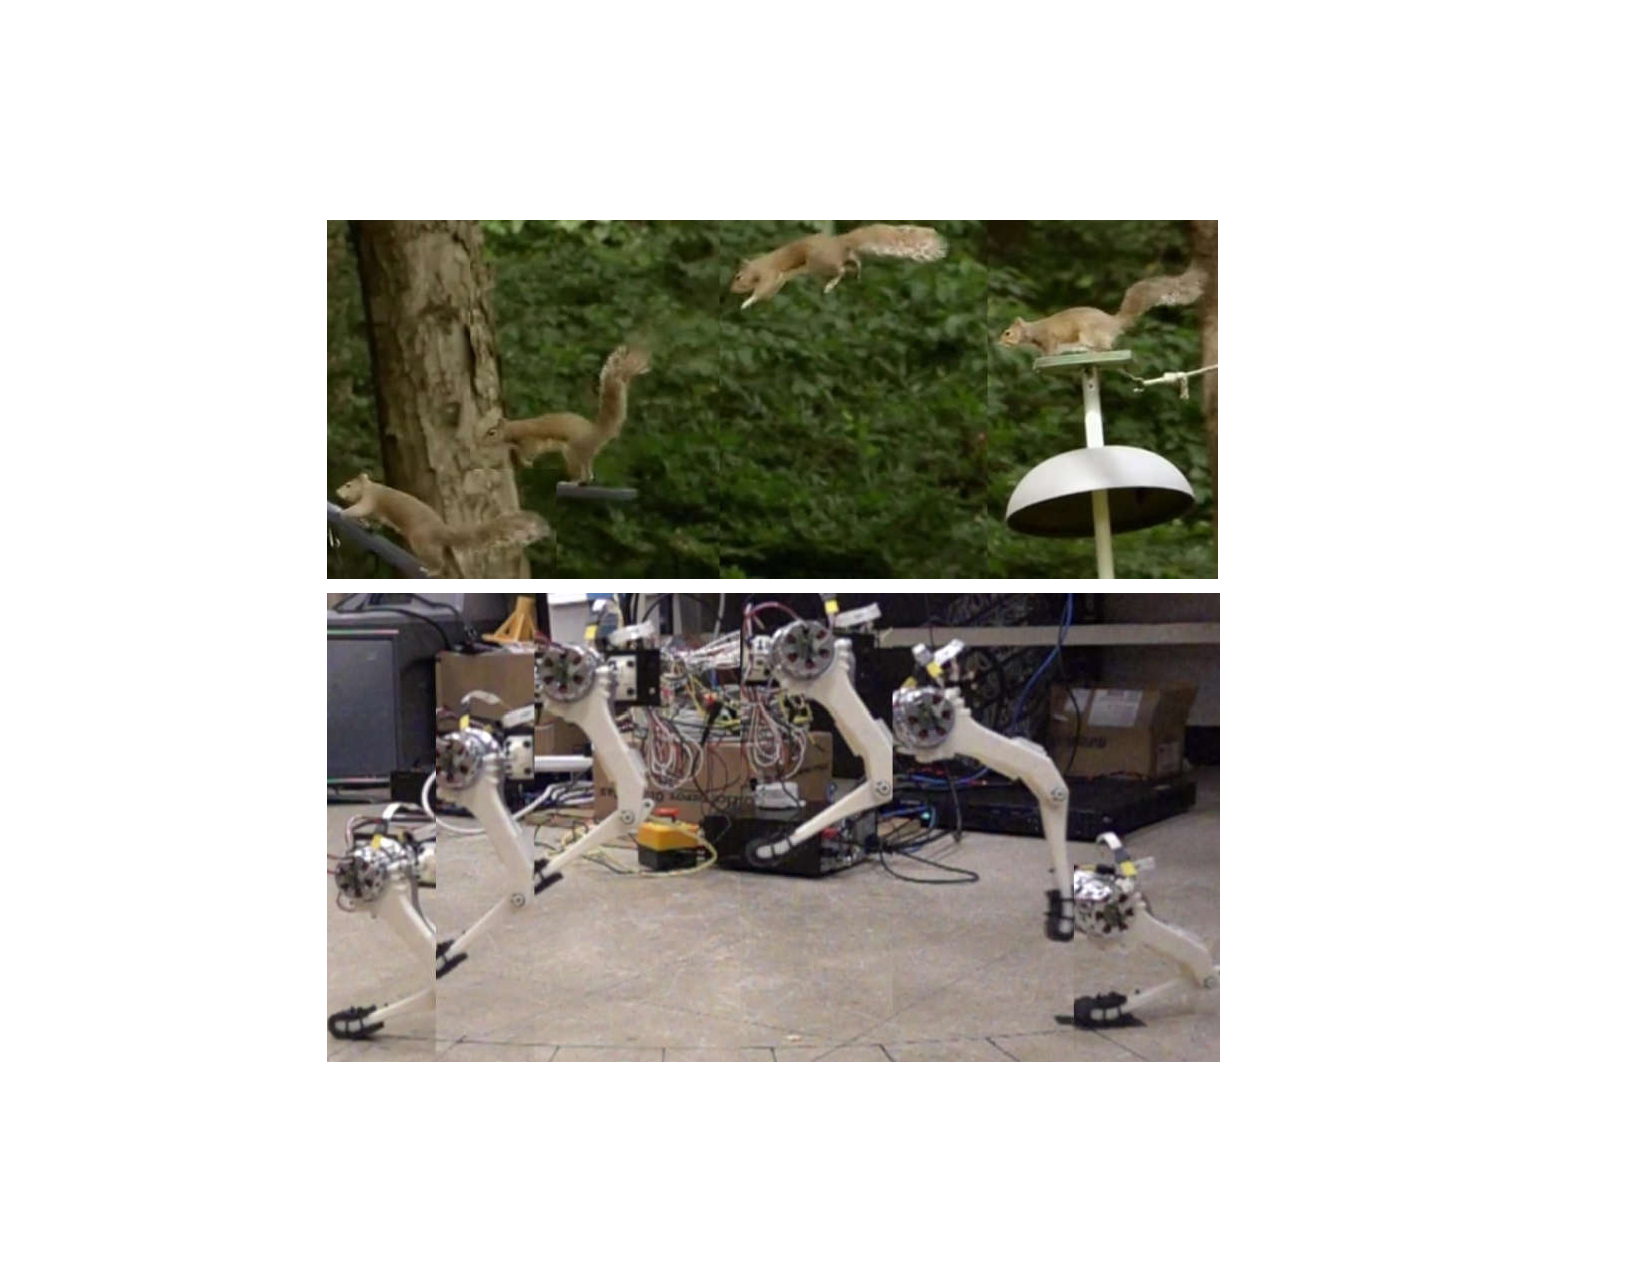
\includegraphics{both_jump.pdf}}
	\caption{A squirrel leaping forward (up) The robot leg presented in this leaping forward (bottom)}
	\label{fig:both_jump}
\end{figure}


\section{Contribution}
\label{sec:contribution}

\section{Thesis Outline}
\label{sec:outline}


